\let\lesson\undefined
\newcommand{\lesson}{\phantomlesson{Bài 7: Phương trình trạng thái của khí lí tưởng}}
\chapter[Bài tập về khí lí tưởng]{Bài tập về khí lí tưởng}
\section{Ôn tập lý thuyết}
\subsection{Phương trình trạng thái}
Phương trình trạng thái khí lí tưởng:
$$\dfrac{pV}{T}=\text{hằng số}.$$
\subsection{Phương trình Clapeyron - Mendeleev}
$$pV=nRT$$
với:
\begin{itemize}
	\item $p$: áp suất khí, đơn vị trong hệ SI là $\si{\pascal}$;
	\item $V$: thể tích khí, đơn vị trong hệ SI là $\si{\meter^3}$;
	\item $n$: số mol khí, đơn vị trong hệ SI là $\si{\mole}$;
	\item $R\approx\SI{8.31}{\dfrac{\joule}{\mole\cdot\kelvin}}$: hằng số khí lí tưởng;
	\item $T$: nhiệt độ tuyệt đối của khí, đơn vị trong hệ SI là $\si{\kelvin}$.
\end{itemize}
\subsection{Các đẳng quá trình}
\begin{center}
	\begin{tabular}{|C{4.5cm}|C{4.5cm}|C{4.5cm}|}
		\hline
		\thead{Đẳng nhiệt\\ $\left(T=const\right)$} &\thead{Đẳng tích\\ $\left(V=const\right)$}& \thead{Đẳng áp\\ $\left(p=const\right)$}\\
		\hline
		&&\\
		$pV=const\Rightarrow p_1V_1=p_2V_2$ & $\dfrac{p}{T}=const\Rightarrow \dfrac{p_1}{T_1}=\dfrac{p_2}{T_2}$ & $\dfrac{V}{T}=const\Rightarrow \dfrac{V_1}{T_1}=\dfrac{V_2}{T_2}$\\[18pt]
		\hline
	\end{tabular}
\end{center}
\subsection{Đồ thị biểu diễn các đẳng quá trình trong các hệ toạ độ}
\subsubsection{Quá trình đẳng nhiệt}
\begin{minipage}{0.3\textwidth}
	\begin{center}
		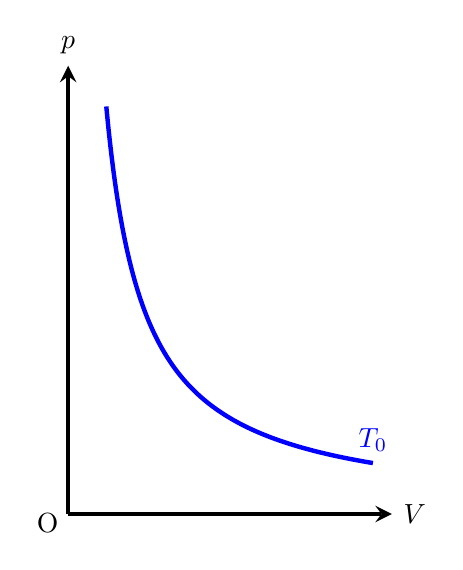
\begin{tikzpicture}  
			\begin{axis}[  ultra thick,xscale=0.6,
				xmin=0,  
				xmax=8.5,  
				xtick=\empty,
				ytick=\empty,
				ymin=0,  
				ymax=2.2, 
				samples=300,
				xticklabels=\empty,
				yticklabels=\empty,
				axis lines=center, 
				xlabel=$V$, 
				ylabel=$p$, 
				every axis y label/.style={at=(current axis.above origin),anchor=south},  
				every axis x label/.style={at=(current axis.right of origin),anchor=west},  ]
				\addplot [ultra thick, blue, smooth, domain=1:8] {2/x} node[above] {$T_0$}; 
			\end{axis}  
			\node[label={[below left]90:O}] at (0,0){};
		\end{tikzpicture}
	\end{center}
\end{minipage}\hfill
\begin{minipage}{0.3\textwidth}
	\begin{center}
		\begin{tikzpicture}  
			\begin{axis}[  ultra thick,xscale=0.6,
				xmin=0,  
				xmax=8.5,  
				xtick={6},
				ytick=\empty,
				ymin=0,  
				ymax=2.2, 
				samples=300,
				xticklabels={$T_0$},
				yticklabels=\empty,
				axis lines=center, 
				xlabel=$T$, 
				ylabel=$p$, 
				every axis y label/.style={at=(current axis.above origin),anchor=south},  
				every axis x label/.style={at=(current axis.right of origin),anchor=west},  ]
				\draw[ultra thick,blue,dashed] (axis cs: 6,0)--(axis cs: 6,0.2); 
				\draw[ultra thick,blue] (axis cs: 6,0.2)--(axis cs: 6,2);
			\end{axis}  
			\node[label={[below left]90:O}] at (0,0){};
		\end{tikzpicture}
	\end{center}
\end{minipage}\hfill
\begin{minipage}{0.3\textwidth}
	\begin{center}
		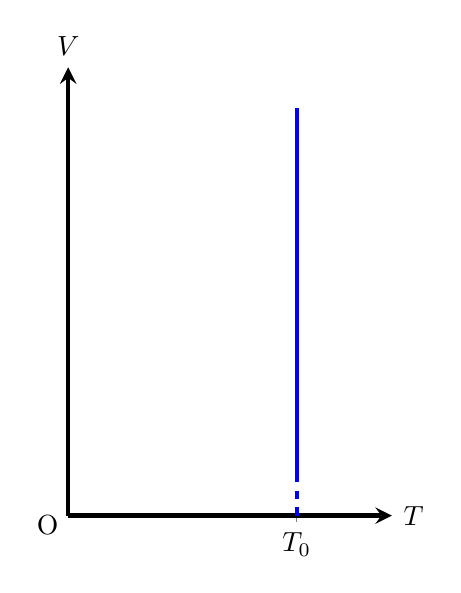
\begin{tikzpicture}  
			\begin{axis}[  ultra thick,xscale=0.6,
				xmin=0,  
				xmax=8.5,  
				xtick={6},
				ytick=\empty,
				ymin=0,  
				ymax=2.2, 
				samples=300,
				xticklabels={$T_0$},
				yticklabels=\empty,
				axis lines=center, 
				xlabel=$T$, 
				ylabel=$V$, 
				every axis y label/.style={at=(current axis.above origin),anchor=south},  
				every axis x label/.style={at=(current axis.right of origin),anchor=west},  ]
				\draw[ultra thick,blue,dashed] (axis cs: 6,0)--(axis cs: 6,0.2); 
				\draw[ultra thick,blue] (axis cs: 6,0.2)--(axis cs: 6,2);
			\end{axis}  
			\node[label={[below left]90:O}] at (0,0){};
		\end{tikzpicture}
	\end{center}
\end{minipage}
\subsubsection{Quá trình đẳng tích}
\begin{minipage}{0.3\textwidth}
	\begin{center}
		\begin{tikzpicture}  
			\begin{axis}[  ultra thick,xscale=0.6,
				xmin=0,  
				xmax=8.5,  
				xtick={6},
				ytick=\empty,
				ymin=0,  
				ymax=2.2, 
				samples=300,
				xticklabels={$V_0$},
				yticklabels=\empty,
				axis lines=center, 
				xlabel=$V$, 
				ylabel=$p$, 
				every axis y label/.style={at=(current axis.above origin),anchor=south},  
				every axis x label/.style={at=(current axis.right of origin),anchor=west},  ]
				\draw[ultra thick,blue,dashed] (axis cs: 6,0)--(axis cs: 6,0.2); 
				\draw[ultra thick,blue] (axis cs: 6,0.2)--(axis cs: 6,2);
			\end{axis}  
			\node[label={[below left]90:O}] at (0,0){};
		\end{tikzpicture}
	\end{center}
\end{minipage}\hfill
\begin{minipage}{0.3\textwidth}
	\begin{center}
		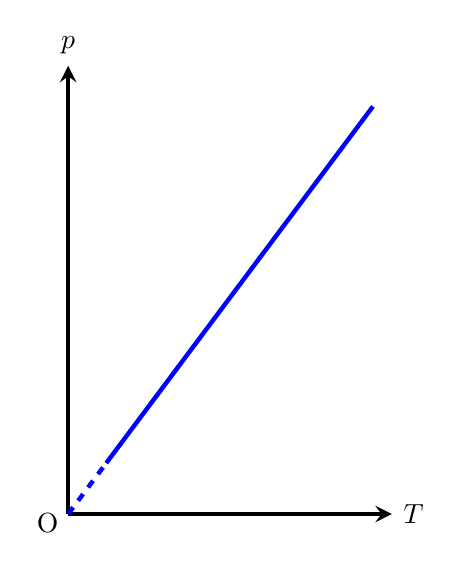
\begin{tikzpicture}  
			\begin{axis}[  ultra thick,xscale=0.6,
				xmin=0,  
				xmax=8.5,  
				xtick=\empty,
				ytick=\empty,
				ymin=0,  
				ymax=2.2, 
				samples=300,
				xticklabels=\empty,
				yticklabels=\empty,
				axis lines=center, 
				xlabel=$T$, 
				ylabel=$p$, 
				every axis y label/.style={at=(current axis.above origin),anchor=south},  
				every axis x label/.style={at=(current axis.right of origin),anchor=west},  ]
				\addplot [ultra thick, blue,dashed, smooth, domain=0:1] {0.25*x}; 
				\addplot [ultra thick, blue, smooth, domain=1:8] {0.25*x}; 
			\end{axis}  
			\node[label={[below left]90:O}] at (0,0){};
		\end{tikzpicture}
	\end{center}
\end{minipage}\hfill
\begin{minipage}{0.3\textwidth}
	\begin{center}
		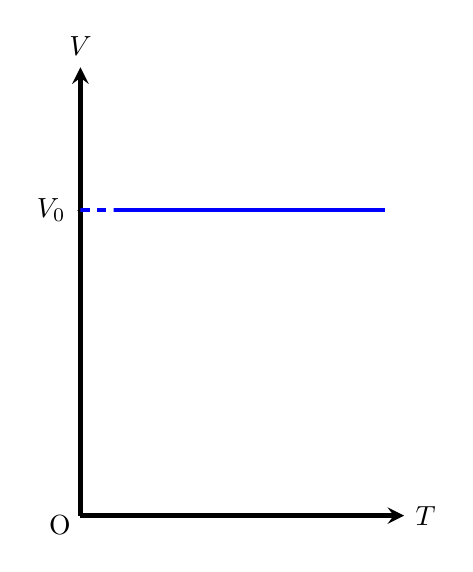
\begin{tikzpicture}  
			\begin{axis}[  ultra thick,xscale=0.6,
				xmin=0,  
				xmax=8.5,  
				xtick=\empty,
				ytick={1.5},
				ymin=0,  
				ymax=2.2, 
				samples=300,
				xticklabels=\empty,
				yticklabels={$V_0$},
				axis lines=center, 
				xlabel=$T$, 
				ylabel=$V$, 
				every axis y label/.style={at=(current axis.above origin),anchor=south},  
				every axis x label/.style={at=(current axis.right of origin),anchor=west},  ]
				\addplot [ultra thick, blue,dashed, smooth, domain=0:1] {1.5}; 
				\addplot [ultra thick, blue, smooth, domain=1:8] {1.5}; 
			\end{axis}  
			\node[label={[below left]90:O}] at (0,0){};
		\end{tikzpicture}
	\end{center}
\end{minipage}
\subsubsection{Quá trình đẳng áp}
\begin{minipage}{0.3\textwidth}
	\begin{center}
		\begin{tikzpicture}  
			\begin{axis}[  ultra thick,xscale=0.6,
				xmin=0,  
				xmax=8.5,  
				xtick=\empty,
				ytick={1.5},
				ymin=0,  
				ymax=2.2, 
				samples=300,
				xticklabels=\empty,
				yticklabels={$p_0$},
				axis lines=center, 
				xlabel=$V$, 
				ylabel=$p$, 
				every axis y label/.style={at=(current axis.above origin),anchor=south},  
				every axis x label/.style={at=(current axis.right of origin),anchor=west},  ]
				\addplot [ultra thick, blue,dashed, smooth, domain=0:1] {1.5}; 
				\addplot [ultra thick, blue, smooth, domain=1:8] {1.5};
			\end{axis}  
			\node[label={[below left]90:O}] at (0,0){};
		\end{tikzpicture}
	\end{center}
\end{minipage}\hfill
\begin{minipage}{0.3\textwidth}
	\begin{center}
		\begin{tikzpicture}  
			\begin{axis}[  ultra thick,xscale=0.6,
				xmin=0,  
				xmax=8.5,  
				xtick=\empty,
				ytick={1.5},
				ymin=0,  
				ymax=2.2, 
				samples=300,
				xticklabels=\empty,
				yticklabels={$p_0$},
				axis lines=center, 
				xlabel=$T$, 
				ylabel=$p$, 
				every axis y label/.style={at=(current axis.above origin),anchor=south},  
				every axis x label/.style={at=(current axis.right of origin),anchor=west},  ]
				\addplot [ultra thick, blue,dashed, smooth, domain=0:1] {1.5}; 
				\addplot [ultra thick, blue, smooth, domain=1:8] {1.5};
			\end{axis}  
			\node[label={[below left]90:O}] at (0,0){};
		\end{tikzpicture}
	\end{center}
\end{minipage}\hfill
\begin{minipage}{0.3\textwidth}
	\begin{center}
		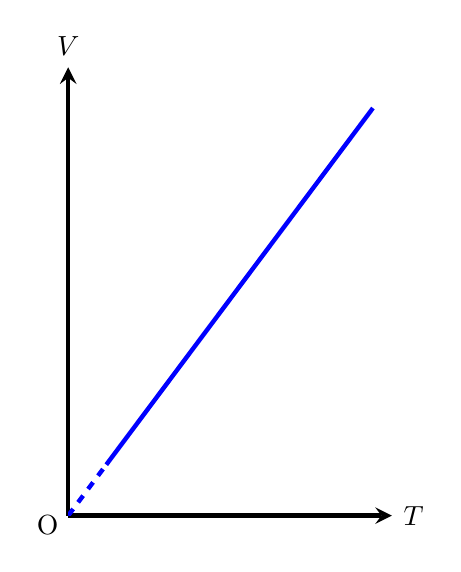
\begin{tikzpicture}  
			\begin{axis}[  ultra thick,xscale=0.6,
				xmin=0,  
				xmax=8.5,  
				xtick=\empty,
				ytick=\empty,
				ymin=0,  
				ymax=2.2, 
				samples=300,
				xticklabels=\empty,
				yticklabels=\empty,
				axis lines=center, 
				xlabel=$T$, 
				ylabel=$V$, 
				every axis y label/.style={at=(current axis.above origin),anchor=south},  
				every axis x label/.style={at=(current axis.right of origin),anchor=west},  ]
				\addplot [ultra thick, blue,dashed, smooth, domain=0:1] {0.25*x}; 
				\addplot [ultra thick, blue, smooth, domain=1:8] {0.25*x}; 
			\end{axis}  
			\node[label={[below left]90:O}] at (0,0){};
		\end{tikzpicture}
	\end{center}
\end{minipage}
\section{Mục tiêu bài học - Ví dụ minh hoạ}
\begin{dang}{Vẽ lại được đồ thị biến đổi trạng thái trong các hệ toạ độ.}
	\viduii{2}
	{Hình bên là đồ thị biểu diễn quá trình biến đổi trạng thái của một lượng khí lí tưởng xác định trong hệ trục toạ độ $OpT$. Hãy biểu diễn các quá trình trên trong hệ trục toạ độ $OpV$ và $OVT$.
		\begin{center}
			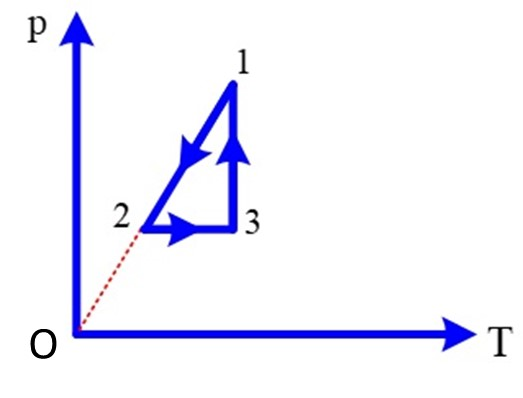
\includegraphics[width=0.25\linewidth]{../figs/VN12-Y24-PH-SYL-014-2}
		\end{center}
	
}
{\hide{\begin{itemize}
		\item Quá trình (1) đến (2) là quá trình đẳng tích: $T$ giảm, $p$ giảm.
		\item Quá trình (2) đến (3) là quá trình đẳng áp: $T$ tăng, $V$ tăng.
		\item Quá trình (3) đến (1) là quá trình đẳng nhiệt: $V$ giảm, $p$ tăng.
	\end{itemize}
\begin{center}
	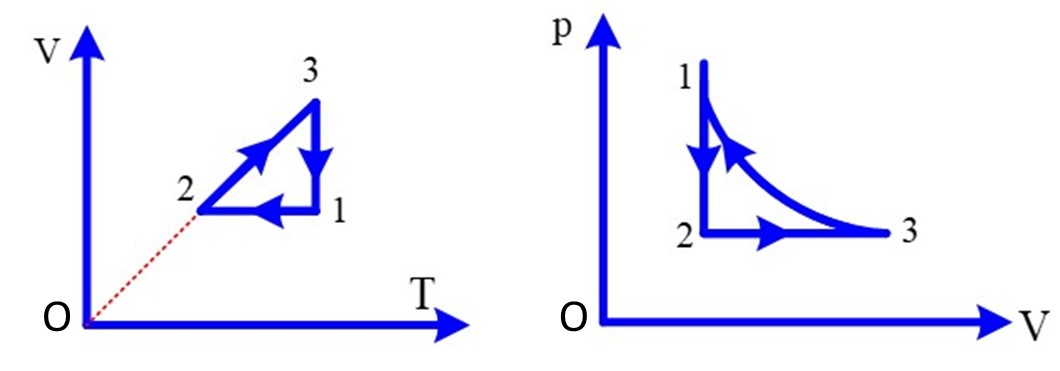
\includegraphics[width=0.65\linewidth]{../figs/VN12-Y24-PH-SYL-014-3}
\end{center}

}}
\end{dang}
\begin{dang}{Dựa vào đồ thị xác định được các thông số trạng thái của khối khí}
	\viduii{3}
	{Một lượng khí helium $\left(\mu=\SI{4}{\gram/\mole}\right)$ có khối lượng $m=\SI{1.0}{\gram}$, nhiệt độ $t_1=\SI{127}{\celsius}$ và thể tích $V_1=\SI{4.0}{\text{lít}}$ biến đổi qua hai giai đoạn:
		\begin{itemize}
			\item Đẳng nhiệt, thể tích tăng gấp hai lần.
			\item Đẳng áp, thể tích trở về giá trị ban đầu.
		\end{itemize}
		\begin{enumerate}[label=\alph*)]
			\item Vẽ đồ thị biểu diễn các quá trình biến đổi trong hệ toạ độ $\left(p, T\right)$.
			\item Tìm nhiệt độ và áp suất thấp nhất trong quá trình biến đổi.
		\end{enumerate}
		
	}
	{\hide{\begin{enumerate}[label=\alph*)]
			\item Các quá trình biến đổi:
			\begin{itemize}
				\item Quá trình $(1)\rightarrow (2)$: quá trình đẳng nhiệt, áp suất tỉ lệ nghịch với thể tích. Thể tích tăng gấp 2 lần $\left(V_2=2V_1\right)$ thì áp suất giảm 2 lần, $p_1=2p_2$.
				\item Quá trình $(2)\rightarrow(3)$: quá trình đẳng áp sao cho $V_3=V_1$. Như vậy, $(3)\rightarrow(1)$ là đường đẳng tích.
			\end{itemize}
			\begin{center}
				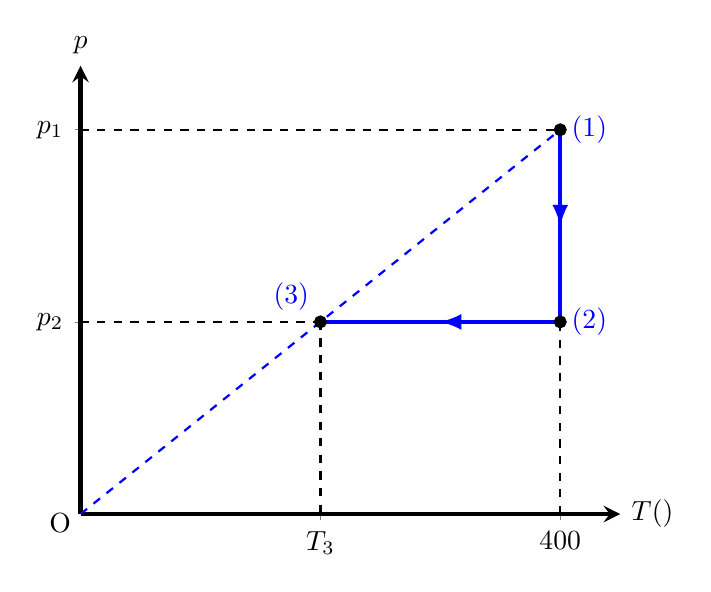
\begin{tikzpicture}  
					\begin{axis}[  ultra thick,
						xmin=0,  
						xmax=450,  
						xtick={200,400},
						ytick={3,6},
						ymin=0,  
						ymax=7, 
						samples=300,
						xticklabels={$T_3$,400},
						yticklabels={$p_2$, $p_1$},
						axis lines=center, 
						xlabel=$\xsi{T}{\left(\kelvin\right)}$, 
						ylabel=$p$, 
						every axis y label/.style={at=(current axis.above origin),anchor=south},  
						every axis x label/.style={at=(current axis.right of origin),anchor=west},  ]
						\draw[thick, dashed] (axis cs: 200,3)--(axis cs: 200,0);
						\draw[thick, dashed] (axis cs: 0,3)--(axis cs: 200,3);
						\draw[thick, dashed] (axis cs: 400,0)--(axis cs: 400,6);
						\draw[thick, dashed] (axis cs: 0,6)--(axis cs: 400,6);
						\addplot [ultra thick, blue, smooth, domain=400:200] {3}; 
						\addplot [ultra thick, blue,-latex, smooth, domain=400:300] {3}; 
						\addplot [thick, blue,dashed, smooth, domain=0:400] {3*x/200};
						\draw[ultra thick, blue] (axis cs: 400,6)--(axis cs: 400,3);
						\draw[ultra thick,-latex, blue] (axis cs: 400,6)--(axis cs: 400,4.5);
						\node[blue,right] at(axis cs: 400, 6) {(1)};
						\node[blue,right] at(axis cs: 400, 3) {(2)};
						\node[blue,above left] at(axis cs: 200, 3) {(3)};
						\filldraw[black] (axis cs:400,3) circle (1.5pt);
						\filldraw[black] (axis cs:400,6) circle (1.5pt);
						\filldraw[black] (axis cs:200,3) circle (1.5pt);
					\end{axis}  
					\node[label={[below left]90:O}] at (0,0){};
				\end{tikzpicture}
			\end{center}
			\item Trong quá trình biến đổi $(1)\rightarrow(2)\rightarrow(3)$: nhiệt độ thấp nhất là $T_3$ và áp suất thấp nhất là $p_2$.
		\end{enumerate}
		Áp dụng phương trình Clapeyron - Mendeleev:
		$$p_1V_1=\dfrac{m}{M}RT_1\Rightarrow p_1=\dfrac{mRT_1}{M V_1}=\dfrac{\left(\SI{1}{\gram}\right)\cdot\left(\SI{8.31}{\dfrac{\joule}{\mole\cdot\kelvin}}\right)\cdot\left(\SI{400}{\kelvin}\right)}{\left(\SI{4}{\gram/\mole}\right)\cdot\left(\SI{4E-3}{\meter^3}\right)}=\SI{207750}{\pascal}.$$
		Áp dụng định luật Boyle cho quá trình biến đổi $(1)\rightarrow(2)$:
		$$p_2=\dfrac{p_1}{2}=\SI{103875}{\pascal}.$$
		Áp dụng định luật Charles cho quá trình biến đổi $(2)\rightarrow(3)$:
		$$\dfrac{V_3}{T_3}=\dfrac{V_2}{T_2}$$
		Mà $V_3=V_1$ và $V_2=2V_1$:
		$$\Rightarrow T_3=\dfrac{T_2}{2}=\dfrac{\SI{400}{\kelvin}}{2}=\SI{200}{\kelvin}.$$
		Vậy: Trong quá trình biến đổi trạng thái của khối khí thì áp suất thấp nhất trong quá trình biến đổi là $p_\text{min}=p_2=\SI{103875}{\pascal}$, nhiệt độ thấp nhất là $T_\text{min}=T_3=\SI{200}{\kelvin}$.
	}}
	
	\viduii{3}
	{Một lượng khí (khí lí tưởng xác định) biến đổi theo chu trình được biểu diễn bởi đồ thị sau:
		\begin{center}
			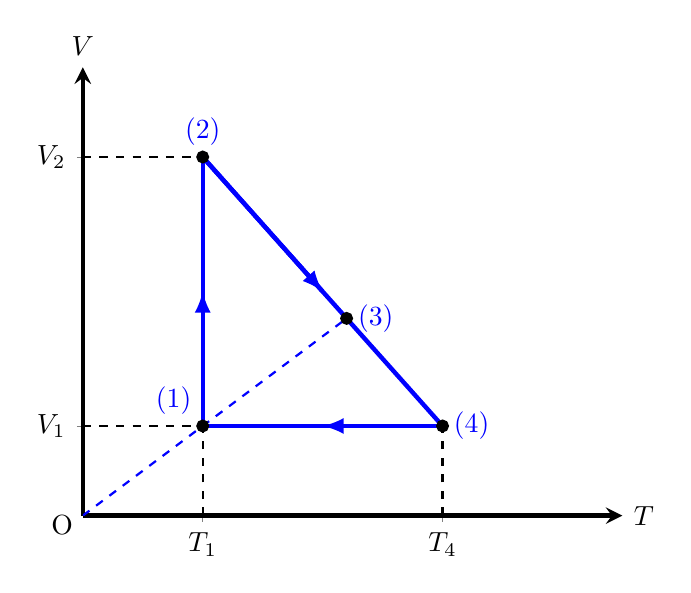
\begin{tikzpicture}  
				\begin{axis}[  ultra thick,
					xmin=0,  
					xmax=450,  
					xtick={100,300},
					ytick={1,4},
					ymin=0,  
					ymax=5, 
					samples=300,
					xticklabels={$T_1$, $T_4$},
					yticklabels={$V_1$, $V_2$},
					axis lines=center, 
					xlabel=$T$, 
					ylabel=$V$, 
					every axis y label/.style={at=(current axis.above origin),anchor=south},  
					every axis x label/.style={at=(current axis.right of origin),anchor=west},  ]
					\draw[thick, dashed] (axis cs: 0,1)--(axis cs: 100,1);
					\draw[thick, dashed] (axis cs: 0,4)--(axis cs: 100,4);
					\draw[thick, dashed] (axis cs: 100,0)--(axis cs: 100,1);
					\draw[thick, dashed] (axis cs: 300,0)--(axis cs: 300,1);
					\addplot [ultra thick, blue, smooth, domain=300:100] {1}; 
					\addplot [ultra thick, blue,-latex, smooth, domain=300:200] {1}; 
					\draw[ultra thick, blue] (axis cs: 100,1)--(axis cs: 100,4);
					\draw[ultra thick,-latex, blue] (axis cs: 100,1)--(axis cs: 100,2.5);
					\draw[ultra thick, blue] (axis cs: 100,4)--(axis cs: 300,1);
					\addplot [ultra thick, blue,-latex, smooth, domain=100:200] {-3*x/200+11/2};
					\addplot [thick, blue,dashed, smooth, domain=0:220] {1*x/100};
					\node[blue,above left] at(axis cs: 100, 1) {(1)};
					\node[blue,above] at(axis cs: 100, 4) {(2)};
					\node[blue,right] at(axis cs: 300, 1) {(4)};
					\node[blue,right] at(axis cs: 220, 2.2) {(3)};
					\filldraw[black] (axis cs:100,1) circle (1.5pt);
					\filldraw[black] (axis cs:100,4) circle (1.5pt);
					\filldraw[black] (axis cs:300,1) circle (1.5pt);
					\filldraw[black] (axis cs:220,2.2) circle (1.5pt);
				\end{axis}  
				\node[label={[below left]90:O}] at (0,0){};
			\end{tikzpicture}
		\end{center}
		Cho biết:\\
		$p_1=p_3$; $V_1=\SI{1}{\meter^3}$; $V_2=\SI{4}{\meter^3}$; $T_1=\SI{100}{\kelvin}$; $T_4=\SI{300}{\kelvin}$. Hãy tìm $V_3$.
	}
	{\hide{\begin{itemize}
			\item Quá trình $(1)\rightarrow(3)$ là quá trình đẳng áp, phương trình đường thẳng $(1)\rightarrow(3)$:
			$$\left(d_{13}\right): V=aT$$
			Khi $T_1=\SI{100}{\kelvin}$ thì $V_1=\SI{1}{\meter^3}$ nên:
			$$a=\dfrac{V_1}{T_1}=\SI{0.01}{\meter^3/\kelvin}\Rightarrow \left(d_{13}\right): V=0,01T\quad\left(\si{\kelvin}, \si{\meter^3}\right).$$
			\item Quá trình $(2)\rightarrow (4)$ có phương trình $V\left(T\right)$ dạng:
			$$\left(d_{24}\right): V=bT+c$$
			Ta có:
			\begin{equation*}
				\begin{cases}
					V_2=bT_2+c\\
					V_4=bT_4+c
				\end{cases}
				\Leftrightarrow
				\begin{cases}
					100b+c=4\\
					400b+c=1
				\end{cases}
				\Rightarrow 
				\begin{cases}
					b=\xsi{-\frac{3}{200}}{\meter^3/\kelvin}\\
					c=\xsi{\frac{11}{2}}{\meter^3}
				\end{cases}
			\end{equation*}
			$\Rightarrow \left(d_{24}\right): V=-\dfrac{3}{200}T+\dfrac{11}{2}\quad \left(\si{\kelvin}, \si{\meter^3}\right).$
			
		\end{itemize}
		Điểm (3) là giao điểm của $\left(d_{13}\right)$ và $\left(d_{24}\right)$:
		\begin{eqnarray*}
			&& \dfrac{V_3}{0,01}=\dfrac{200}{3}\cdot\left(\dfrac{11}{2}-V_3\right)\\
			&\Rightarrow& V_3=\SI{2.2}{\meter^3}.
		\end{eqnarray*}
		Vậy: $V_3=\SI{2.2}{\meter^3}$.
		
	}}
	
\end{dang}